\documentclass[11pt,a4paper]{article}
\usepackage[a4paper,top=21mm,bottom=21mm,left=22mm,right=22mm,headheight=15pt]{geometry}
\usepackage{libertinus,microtype,fancyhdr,titlesec}
\usepackage[hidelinks]{hyperref}
\usepackage[T1]{fontenc}
\usepackage[brazil]{babel}
\usepackage{graphicx,booktabs,tabularx,amsmath,tikz}
\usetikzlibrary{arrows.meta}
\definecolor{Ink}{HTML}{142637}
\definecolor{Teal}{HTML}{176C69}
\definecolor{Rust}{HTML}{9C4028}
\definecolor{Rule}{HTML}{D6E0E9}
\definecolor{Tint}{HTML}{EDF5F4}
\newcommand{\projetourl}{https://github.com/costaleirbag/projeto-mae5920}
\newcommand{\fonte}[2]{\href{\projetourl/blob/51cb94e9b67a05c0a4e0cbb9c6740c51e5821f15/#1}{#2}}
\newcommand{\fonteatual}[2]{\href{\projetourl/blob/main/#1}{#2}}
\newcommand{\nota}[1]{{\small\color{Ink!82}#1}}
\newcommand{\caso}[2]{\noindent\textcolor{Teal}{\sffamily\bfseries #1}\quad\textit{#2}\par}
\newcommand{\Arquitetura}{\resizebox{\linewidth}{!}{\begin{tikzpicture}[
  bloco/.style={draw=Rule,fill=Tint,text=Ink,align=center,minimum height=9mm,
    minimum width=21mm,inner sep=3pt,font=\sffamily\small},
  passo/.style={-{Latex[length=2mm]},draw=Teal,line width=.55pt}
]
  \node[bloco] (ids) at (0,0) {IDs\\\(B\times T\)};
  \node[bloco] (emb) at (2.75,0) {Embedding\\\(B\times T\times128\)};
  \node[bloco] (k3) at (5.65,1.05) {Conv + ReLU\\\(k=3\), 100 filtros};
  \node[bloco] (k4) at (5.65,0) {Conv + ReLU\\\(k=4\), 100 filtros};
  \node[bloco] (k5) at (5.65,-1.05) {Conv + ReLU\\\(k=5\), 100 filtros};
  \node[bloco] (max) at (8.48,0) {Máximo global\\com máscara};
  \node[bloco] (cat) at (11.23,0) {Concatenação\\e dropout\\\(B\times300\)};
  \node[bloco] (out) at (13.9,0) {Linear\\\(B\times2\)};
  \draw[passo] (ids) -- (emb);
  \draw[passo] (emb.east) -- ++(.18,0) |- (k3.west);
  \draw[passo] (emb.east) -- (k4.west);
  \draw[passo] (emb.east) -- ++(.18,0) |- (k5.west);
  \draw[passo] (k3.east) -- ++(.18,0) |- (max.west);
  \draw[passo] (k4.east) -- (max.west);
  \draw[passo] (k5.east) -- ++(.18,0) |- (max.west);
  \draw[passo] (max) -- (cat);
  \draw[passo] (cat) -- (out);
\end{tikzpicture}
}}
% Gerado por preparar.py a partir das evidências publicadas.
\newcommand{\LinhasOriginal}{Treino & TF-IDF + logística & 99,72\% & 0,9972 & 0,0973 \\
Treino & CNN & 94,95\% & 0,9494 & 0,1567 \\
Treino & BERT & 96,32\% & 0,9632 & 0,1138 \\
\addlinespace[2pt]
Validação & TF-IDF + logística & 91,53\% & 0,9152 & 0,2255 \\
Validação & CNN & 87,97\% & 0,8796 & 0,2877 \\
Validação & BERT & 91,28\% & 0,9128 & 0,2404 \\
\addlinespace[2pt]
Teste & TF-IDF + logística & 90,14\% & 0,9014 & 0,2531 \\
Teste & CNN & 86,78\% & 0,8678 & 0,3040 \\
Teste & BERT & 90,94\% & 0,9094 & 0,2433 \\}
\newcommand{\LinhasTeste}{TF-IDF + logística & 90,14\% & 0,9014 & 0,2396 \\
CNN & 86,78\% & 0,8678 & 0,3037 \\
BERT & 90,94\% & 0,9094 & 0,2278 \\}
\newcommand{\PontosTeste}{\officialpoint{33}{TF-IDF + logística}{90.144}{90,14\%}{0,9014}{0,2396}{Quiet}{Resenha inteira}{L2, \(C=8\)}
\officialpoint{20}{CNN}{86.78399999999999}{86,78\%}{0,8678}{0,3037}{Teal}{400 tokens por regex}{0,001 \(\cdot\) lote 64 \(\cdot\) 5 épocas}
\officialpoint{7}{BERT}{90.944}{90,94\%}{0,9094}{0,2278}{Quiet}{192 WordPieces}{0,00002 \(\cdot\) lote 32 \(\cdot\) 2 épocas}}
\newcommand{\KernelsVisuais}{\labvalue{3}{100 filtros}{81,27\%}
\labvalue{5}{100 filtros}{80,94\%}
\labvalue{3/4/5}{300 filtros}{81,95\%}}
\newcommand{\PassosVisuais}{\labvalue{1}{100,0\% das janelas}{82,00\%}
\labvalue{2}{50,2\% das janelas}{81,45\%}
\labvalue{3}{33,6\% das janelas}{80,97\%}}
\newcommand{\RecorteVisual}{\cutrow{Primeiros 400 tokens}{71,7\%}{94,7\%}{Teal}
\cutrow{Texto inteiro}{6,5\%}{12,1\%}{Rust}}
\newcommand{\TrechoPrefixo}{This film is as crassly manipulative as it is vapid}
\newcommand{\PosTrechoPrefixo}{230--239}
\newcommand{\TrechoFinal}{I had to leave because it was so bad.}
\newcommand{\PosTrechoFinal}{716--724}
\newcommand{\SemPosHumanos}{39,8\%}
\newcommand{\ComPosHumanos}{39,1\%}
\newcommand{\NParesHumanos}{344}
\newcommand{\LinhasCusto}{TF-IDF + logística & CPU do Apple M1 & — & 13,1 & 0,15 \\
CNN & Apple M1 (MPS) & 5 & 139,6 & 20,72 \\
BERT & NVIDIA GB10 (CUDA) & 2 & 446,4 & 149,91 \\}
\newcommand{\LinhasCustoSlide}{TF-IDF & M1 CPU & — & 13,1 \\
CNN & M1 GPU & 5 & 139,6 \\
BERT & GB10 GPU & 2 & 446,4 \\}
\newcommand{\AjusteCabecaBert}{17,6}
\newcommand{\AjusteCompletoBert}{148,9}
\newcommand{\AcuraciaCabecaBert}{84,52\%}
\newcommand{\AcuraciaCompletoBert}{88,31\%}
\newcommand{\LinhasSeq}{TF-IDF + logística & 83,30\% & 0,8330 & 0,3849 \\
CNN + Adam & 81,95\% & 0,8194 & 0,4094 \\
BERT-base ajuste completo & 88,31\% & 0,8831 & 0,3027 \\
DistilBERT ajuste completo & 86,80\% & 0,8678 & 0,3382 \\
ModernBERT-base ajuste completo & 91,24\% & 0,9124 & 0,2458 \\}
\newcommand{\LinhasBPE}{Regex por palavras & 82,00\% & 0,8200 & 0,3964 & 3,27\% & 121,3 \\
BPE 20 mil & 81,41\% & 0,8140 & 0,4052 & 0,00\% & 129,1 \\}
\newcommand{\ExemploTFIDF}{Movie was awful.}
\newcommand{\NormaExemploTFIDF}{8,525}
\newcommand{\IDFAwful}{3,845}
\newcommand{\TFIDFAwful}{0,451}
\newcommand{\LinhasExemploTFIDF}{\texttt{movie} & 0,175 & -1,542 & -0,269 \\
\texttt{was} & 0,168 & -3,724 & -0,627 \\
\texttt{awful} & 0,451 & -10,744 & -4,846 \\
\texttt{movie was} & 0,418 & -0,678 & -0,284 \\
\texttt{was awful} & 0,750 & -1,982 & -1,487 \\}
\newcommand{\ViesExemploTFIDF}{+0,211}
\newcommand{\EscoreExemploTFIDF}{-7,302}
\newcommand{\PositivaExemploTFIDF}{0,067\%}
\newcommand{\TfidfControleIntegral}{90,15\%}
\newcommand{\TfidfControleCorte}{89,66\%}
\newcommand{\LinhasPares}{Contraste depois de but & Pos. / Neg. & 1,0\% & 89,9\% & 1,2\% & 83,7\% & 3/3 e 3/3 \\
Escopo de not & Pos. / Neg. & 48,4\% & 10,3\% & 53,1\% & 15,5\% & 2/3 e 1/3 \\
Sentimento por aspecto & Mista / Mista & 29,9\% & 0,3\% & 20,0\% & 0,4\% & 0/3 e 0/3 \\
Troca de blocos com as mesmas janelas & Mista / Mista & 88,4\% & 88,4\% & 73,6\% & 73,6\% & 0/3 e 0/3 \\}
\newcommand{\LinhasForaDominio}{Amazon & 68,10\% & 0,6664 & 0,6372 & 69,97\% & 0,6920 & 0,5900 \\
Yelp & 69,43\% & 0,6828 & 0,6091 & 69,67\% & 0,6911 & 0,5946 \\}
\newcommand{\SoTFIDF}{1.715}
\newcommand{\SoCNN}{875}
\newcommand{\Discordancias}{2.590}
\newcommand{\PassoUm}{82,00\%}
\newcommand{\PassoDois}{81,45\%}
\newcommand{\PassoTres}{80,97\%}
\newcommand{\TextoA}{I thought this movie was terrible, but it was wonderful.}
\newcommand{\TextoB}{I thought this movie was wonderful, but it was terrible.}
\newcommand{\ExemploCobertura}{The pallbearer scene was unexpectedly moving.}
\newcommand{\PalavrasA}{1,0\%}
\newcommand{\PalavrasB}{89,9\%}
\newcommand{\BPEA}{1,2\%}
\newcommand{\BPEB}{83,7\%}
\newcommand{\TfidfContrasteA}{47,93\%}
\newcommand{\TfidfContrasteB}{47,86\%}
\newcommand{\NegacaoPalavrasA}{53,7\%}
\newcommand{\NegacaoBPEA}{47,5\%}
\newcommand{\BPEInicio}{\chip{p}\chip{a}\chip{l}\chip{l}\chip{b}\chip{e}\chip{a}\chip{r}\chip{e}\chip{r</w>}}
\newcommand{\BPEFusao}{\chip{p}\chip{a}\chip{l}\chip{l}\chip{b}\chip{e}\chip{a}\fused{re}\chip{r</w>}}
\newcommand{\BPEFim}{\chip{p}\chip{all}\fused{bearer</w>}}
\newcommand{\FiltroDemo}{89}
\newcommand{\MaximoDemo}{0,98}
\newcommand{\MaximoPassoDois}{0,40}
\newcommand{\JanelaControle}{movie i loved}
\newcommand{\InicioControleA}{8}
\newcommand{\InicioControleB}{20}
\newcommand{\MaximoControle}{0,47}
\newcommand{\FiltroControle}{61}
\newcommand{\PicoPrimeiraMetade}{0,47}
\newcommand{\PicoSegundaMetade}{0,25}
\newcommand{\CnnRoom}{\good{Positiva 6/6}}
\newcommand{\CnnSquad}{\pill{Paper}{Ink}{5 pos. / 1 neg. (BPE, semente 43)}}
\newcommand{\QwenRoomSem}{\good{Positiva 3/3}}
\newcommand{\QwenRoomCom}{\good{Positiva 3/3}}
\newcommand{\QwenSquadSem}{\bad{Negativa 3/3}}
\newcommand{\QwenSquadCom}{\bad{Negativa 3/3}}

% Gerado por preparar_relatorio.py a partir de dados/comprimentos.json.
\newcommand{\LinhasDistribuicao}{Resenha no treino & 19.823 & 10 & 90 & 231,1 & 173 & 451 & 2.459 \\
Resenha no teste & 25.000 & 4 & 88 & 226,2 & 170 & 439 & 2.235 \\
Frase no teste* & 312.557 & 1 & 5 & 18,1 & 16 & 33 & 722 \\}
\newcommand{\LinhasDistribuicaoSlide}{Resenha no treino & 231,1 & 173 & 451 \\
Resenha no teste & 226,2 & 170 & 439 \\
Frase no teste* & 18,1 & 16 & 33 \\}
\newcommand{\LinhasPorComprimento}{Até 100 & 3.246 & 90,73 / 90,67 & 87,34 / 87,23 & 93,10 / 93,03 & 95,19 / 95,17 \\
101 a 250 & 14.624 & 90,15 / 90,15 & 87,45 / 87,45 & 92,97 / 92,97 & 95,34 / 95,34 \\
251 a 500 & 5.285 & 89,74 / 89,73 & 86,45 / 86,44 & 86,93 / 86,92 & 95,40 / 95,40 \\
Acima de 500 & 1.845 & 90,19 / 90,16 & 81,52 / 81,46 & 82,60 / 82,46 & 94,36 / 94,35 \\}
\newcommand{\LinhasPorComprimentoSlide}{Até 100 & 3.246 & 90,7 / 90,7 & 87,3 / 87,2 & 93,1 / 93,0 \\
101 a 250 & 14.624 & 90,2 / 90,2 & 87,4 / 87,4 & 93,0 / 93,0 \\
251 a 500 & 5.285 & 89,7 / 89,7 & 86,5 / 86,4 & 86,9 / 86,9 \\
Acima de 500 & 1.845 & 90,2 / 90,2 & 81,5 / 81,5 & 82,6 / 82,5 \\}
\newcommand{\QuantidadeLongas}{1.845}
\newcommand{\AcuraciaLongasCNN}{81,52\%}
\newcommand{\AcuraciaLongasCNNIntegral}{86,18\%}
\newcommand{\BertTetoOriginal}{192}
\newcommand{\BertTetoMaior}{512}
\newcommand{\FUmLongasBert}{82,46\%}
\newcommand{\FUmLongasBertMaior}{89,69\%}


\hypersetup{colorlinks=true,linkcolor=Teal,urlcolor=Teal,citecolor=Teal,
  pdftitle={O que a CNN lê em uma resenha?},pdfauthor={Nestor, Letícia e Gabriel}}
\color{Ink}
\setlength{\parindent}{0pt}
\setlength{\parskip}{5pt plus 1pt minus 1pt}
\setlength{\emergencystretch}{2em}
\renewcommand{\arraystretch}{1.14}
\setcounter{secnumdepth}{2}
\titleformat{\section}{\Large\sffamily\bfseries\color{Ink}}{\textcolor{Teal}{\thesection}}{.65em}{}
\titleformat{\subsection}{\normalsize\sffamily\bfseries\color{Teal}}{}{0pt}{}
\titlespacing*{\section}{0pt}{8pt}{6pt}
\titlespacing*{\subsection}{0pt}{8pt}{3pt}
\pagestyle{fancy}
\fancyhf{}
\fancyhead[L]{\footnotesize\sffamily MAE5920\enspace$\cdot$\enspace Introdução a Deep Learning}
\fancyhead[R]{\footnotesize\sffamily CNN e tokenização}
\fancyfoot[R]{\footnotesize\sffamily\thepage}
\renewcommand{\headrulewidth}{.4pt}
\newcommand{\legendinha}[1]{\par\vspace{3pt}{\footnotesize #1\par}}
\newcommand{\tabelahead}[1]{\leavevmode{\sffamily\bfseries\color{Teal}#1}}
\begin{document}
\thispagestyle{empty}
\vspace*{8mm}
{\sffamily\bfseries\color{Teal} MAE5920\enspace $\cdot$\enspace INTRODUÇÃO A DEEP LEARNING\par}
\vspace{5mm}
{\fontsize{34}{37}\selectfont\sffamily\bfseries O que a CNN lê\\ em uma resenha?\par}
\vspace{3mm}
{\large Classificação de sentimento e tokenização no IMDb\par}
\vspace{5mm}
{\sffamily Nestor, Letícia e Gabriel\par}
\vspace{6mm}
\noindent\textcolor{Rule}{\rule{\linewidth}{.7pt}}

\subsection*{Resumo}
Classificamos resenhas do IMDb em positivas e negativas com regressão logística
sobre TF-IDF, uma CNN com embeddings aprendidos e encoders pré-treinados.
O experimento original avalia os modelos no teste oficial. Ensaios internos
com três sementes separam escolhas de otimizador, arquitetura e tokenização.
Na comparação pareada, BPE reduziu tokens desconhecidos de 3,27\% para zero e
a acurácia média passou de 82,00\% para 81,41\%. Em um par sintético com as mesmas
palavras, as duas CNNs mudaram de classe quando trocamos a ordem dos adjetivos.
Os seis checkpoints inverteram a interpretação prevista para as duas frases.
Um controle com as mesmas janelas convolucionais produziu logits idênticos
em cada checkpoint. Esses exemplos ajudam a localizar o que a arquitetura
consegue distinguir, mesmo quando o desempenho agregado parece semelhante.

\section{Ordem e sentimento}
\label{sec:ordem}
Considere duas resenhas que só trocam os lugares de \textit{terrible} e
\textit{wonderful}. A oração após \textit{but} expressa a avaliação final.

\vspace{2mm}
\caso{A}{\TextoA}
\caso{B}{\TextoB}
\vspace{1mm}
As duas sequências têm a mesma contagem de cada palavra. Um modelo que recebe
apenas unigramas vê o mesmo vetor para A e B. Os bigramas mudam, portanto o
TF-IDF de referência deste trabalho, que inclui bigramas, pode separá-las.
A CNN também pode responder de modo diferente, pois aplica filtros a janelas
ordenadas de embeddings. A questão empírica é se ela atribui o sentimento à
oração que encerra o contraste.

Investigamos essa questão em três escalas. Primeiro, medimos desempenho em
resenhas reservadas. Depois, alteramos componentes da CNN sob controles de
treino e avaliamos palavras contra subpalavras. Por fim, consultamos pesos
congelados com pares sintéticos para verificar sensibilidade à ordem e
construir um limite exato da arquitetura.

\vfill
\nota{Código, notebook executado e resultados por execução.
\href{\projetourl}{Repositório do projeto}.}

\newpage
\section{Dados e protocolo de avaliação}
\label{sec:dados}
O IMDb tem 25.000 resenhas em inglês no treino oficial e 25.000 no teste
\cite{maas}, com rótulos \(0\) (negativo) e \(1\) (positivo). A limpeza
decodifica HTML, remove tags e normaliza espaços em cada texto.

\subsection{Papéis das amostras}
\begin{tabularx}{\linewidth}{@{}lrrX@{}}
\toprule
\tabelahead{Papel} & \tabelahead{Original} & \tabelahead{Ensaios internos} & \tabelahead{Uso}\\
\midrule
Treino       & 19.823 & 6.144 & Ajustar representação, vocabulário e pesos.\\
Validação    &  2.478 & 1.536 & Escolher hiperparâmetros e época.\\
Calibração   &  2.478 &  --   & Ajustar temperatura após a seleção original.\\
Teste/auditoria & 25.000 & 2.048 & Avaliar a configuração já escolhida.\\
\bottomrule
\end{tabularx}
\legendinha{Tabela 1. Cada extensão tem auditoria própria, aberta após
congelar pesos e escolhas.}

Os ensaios internos com sequências usam até 128 palavras. Na auditoria
BPE, esse teto cortou 1.535 resenhas e manteve 51,24\% dos tokens por
palavras. Os prefixos já cabiam no teto adicional de 256 tokens.
\fonte{docs/PROTOCOLO_SEQUENCIAS.md}{Protocolo sequencial} e
\fonte{docs/PROTOCOLO_BPE.md}{protocolo BPE}.

\subsection{Comprimento antes dos recortes}
{\small
\begin{tabularx}{\linewidth}{@{}Xrrrrrrr@{}}
\toprule
\tabelahead{Unidade} & \tabelahead{\(n\)} & \tabelahead{Mín.} & \tabelahead{P10} &
\tabelahead{Média} & \tabelahead{Mediana} & \tabelahead{P90} & \tabelahead{Máx.}\\
\midrule
\LinhasDistribuicao
\bottomrule
\end{tabularx}}
\legendinha{Tabela 2. Palavras separadas por espaços no texto limpo.
*Frases estimadas por pontuação final. \fonteatual{seminario/dados/comprimentos.json}{Distribuições completas}.}

\subsection{Análise de possíveis vazamentos de informação}
Removemos 123 linhas do treino com hash presente no teste e 98 duplicatas
internas, usando SHA-256 do texto limpo com \textit{casefold}. Para excluir
duplicatas, lemos o texto do teste e reservamos os rótulos à avaliação.
Os quatro conjuntos finais têm zero hashes em comum. O teste conserva
201 ocorrências duplicadas. \fonte{data/manifest.json}{Manifesto}.

Ajustamos TF-IDF, vocabulário da CNN e fusões do BPE no treino. A checagem
cobre igualdade de texto, e paráfrases ou exposição no pré-treino seguem
em aberto. A análise de erros e o Qwen reutilizam o teste em caráter exploratório.

\subsection{Dicionário de dados resumido}
\begin{tabularx}{\linewidth}{@{}lX@{}}
\toprule
\tabelahead{Campo} & \tabelahead{Significado}\\
\midrule
\texttt{id} & Identificador derivado da divisão oficial e da posição na fonte.\\
\texttt{label} & Classe binária usada na função de perda e na avaliação.\\
\texttt{clean\_text} & Texto após decodificação de HTML e normalização de espaços.\\
\texttt{word\_count} & Número de segmentos separados por espaço no texto limpo.\\
\texttt{text\_sha256} & Impressão do texto normalizado usada para verificar duplicações.\\
\bottomrule
\end{tabularx}
\legendinha{Tabela 3. A única entrada do classificador é o texto.
\fonte{DATA_DICTIONARY.md}{Dicionário completo}.}

\subsection{Métricas}
Acurácia é a fração de acertos. F1 macro dá o mesmo peso ao F1 de cada
classe. A entropia cruzada (CE) é a média de \(-\log p(\text{classe verdadeira})\).

\newpage
\section{Tokenização e arquitetura}
\label{sec:arquitetura}
\subsection{Duas unidades de entrada}
\textbf{Palavras.} Convertemos o prefixo limpo para minúsculas. A expressão
\verb|[a-z]+(?:'[a-z]+)?|\verb!|\d+! preserva palavras, contrações e números.
O vocabulário contém os 19.998 itens mais frequentes no treino, além de
\texttt{<pad>} (ID 0) e \texttt{<unk>} (ID 1). A frequência determina a ordem,
com desempate lexical. A posição de cada ID é preservada na sequência.
Palavras de negação como \textit{not} seguem para o modelo.

\textbf{BPE.} Mantemos a normalização lexical e separamos palavras com
\texttt{WhitespaceSplit}. O BPE de caracteres aprende uniões de pares
frequentes com os 6.144 textos de treino, frequência mínima 2 e vocabulário
de 20.000 itens. O marcador \texttt{</w>} identifica o fim de palavra.
O tokenizer é congelado antes do treino supervisionado da CNN.
O procedimento adapta BPE para unidades de texto \cite{sennrich}.

\caso{Entrada}{\ExemploCobertura}
\begin{tabularx}{\linewidth}{@{}lX@{}}
\toprule
\tabelahead{Palavras} & \texttt{the \enspace <unk> \enspace scene \enspace was \enspace unexpectedly \enspace moving}\\
\tabelahead{BPE} & \texttt{the</w> \enspace p \enspace all \enspace bearer</w> \enspace scene</w>} \newline
\texttt{was</w> \enspace unexpectedly</w> \enspace moving</w>}\\
\bottomrule
\end{tabularx}
\legendinha{Tabela 3. Saída dos tokenizadores congelados. \texttt{pallbearer} tem
um ID desconhecido com palavras e três peças com BPE.}

\subsection{Convolução sobre embeddings}
Cada ID acessa um vetor de 128 dimensões aprendido com a tarefa. O filtro
de largura \(k\) lê \(k\) tokens vizinhos e usa os mesmos pesos em todas as
posições. Aplicamos três grupos paralelos de convoluções de larguras 3, 4 e
5, com cem filtros por largura. A ReLU deixa respostas positivas passarem.
O máximo global seleciona a maior ativação por filtro. A topologia segue
a família de CNNs para classificação de sentenças \cite{kim,prince}.

\vspace{2mm}
\Arquitetura
\legendinha{Figura 1. TextCNN do projeto. \(B\) é o tamanho do minibatch e \(T\) é
o comprimento após padding. A camada linear produz logits negativo e positivo.}

Se \(e_t\) é o embedding na posição \(t\), o filtro \(f\) resume a entrada por
\[
  m_f = \max_{t\in\mathcal V_k}
  \operatorname{ReLU}\!\left(\langle W_f, [e_t,\ldots,e_{t+k-1}]\rangle + b_f\right).
\]
\(\mathcal V_k\) exclui as janelas que avançam sobre padding em entradas com
pelo menos \(k\) tokens. Para sequências mais curtas, a implementação mantém
a primeira janela com padding. A concatenação dos 300 máximos passa por dropout de
0,5 no treino e uma camada \(\mathrm{Linear}(300,2)\).

Na CNN principal, \(20.000\times128=2.560.000\) parâmetros pertencem aos
embeddings. As convoluções somam \(100\sum_{k\in\{3,4,5\}}(128k+1)=153.900\).
A saída soma \(2(300+1)=602\), totalizando \textbf{2.714.502 parâmetros}.
A mesma largura em tokens pode abranger menos palavras quando BPE fragmenta
uma palavra. \fonte{src/imdb_lab/models.py}{Implementação}.

\newpage
\section{O que mudou durante o treino}
\label{sec:treino}
Em cada minibatch, a rede produz dois logits por resenha e a entropia
cruzada mede a perda frente ao rótulo. O \textit{backward} calcula os
gradientes dos embeddings, filtros e saída. Limitamos sua norma global a
1 antes da atualização. Os embeddings começam com distribuição normal de
desvio 0,1 e linha de padding zero. Os filtros usam inicialização de He
e a saída, Xavier \cite{prince}.

\subsection{Como escolhemos a taxa e a época}
\begin{tabularx}{\linewidth}{@{}lXr@{}}
\toprule
\tabelahead{Otimizador} & \tabelahead{Taxas testadas} & \tabelahead{Escolhida}\\
\midrule
SGD & 0,001 \quad 0,03 \quad 0,3 & 0,3\\
SGD com momentum 0,9 & 0,001 \quad 0,01 \quad 0,1 & 0,1\\
Adam & 0,0003 \quad 0,001 \quad 0,003 & 0,001\\
\bottomrule
\end{tabularx}
\legendinha{Tabela 3. Três sementes por célula (17, 29 e 43), minibatches de
64 e orçamento de 12 épocas. A CNN base tem larguras 3/4/5, cem filtros por
largura e dropout de 0,5.}

Na mesma semente, fixamos pesos iniciais e ordem dos minibatches. Salvamos
a época de menor CE de validação de cada treino e escolhemos a taxa com a
menor média dessa perda entre sementes. A época zero é a inicialização.

\medskip
\noindent\makebox[\linewidth]{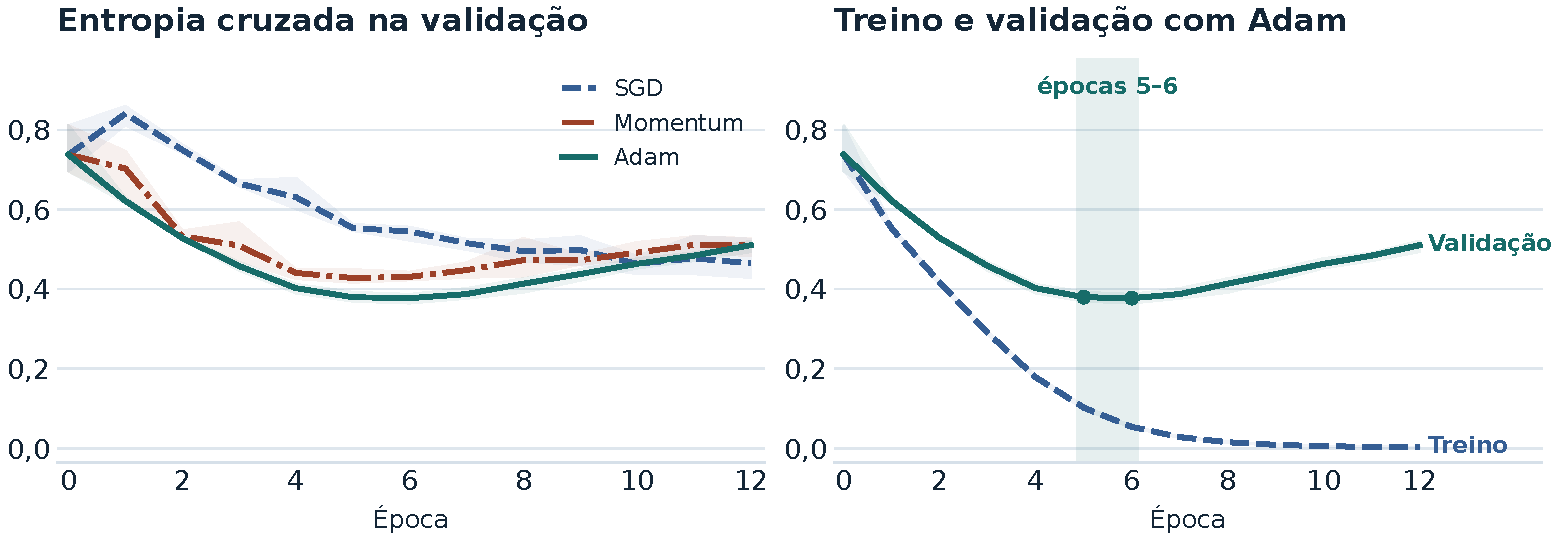
\includegraphics[width=.89\linewidth]{figuras/otimizacao.pdf}}
\legendinha{Figura 2. As linhas são médias e as faixas cobrem mínimo e máximo
entre sementes. À esquerda, cada otimizador usa sua taxa escolhida. À direita,
a perda de treino com Adam continua caindo depois da melhor região de
validação. Os checkpoints de Adam vêm das épocas 5 e 6.}

\subsection{Largura, número de filtros e dropout}
Fizemos 42 treinos de CNN. Além dos 27 acima, nove variaram largura ou
número de filtros e seis variaram dropout. Na auditoria sequencial,
larguras 3 e 5 isoladas (100 filtros) chegaram a 81,27\% e 80,94\% de
acurácia. A combinação 3/4/5 chegou a 81,95\% com 300 filtros e a
81,64\% com 96. Com dropout de 0,8, a acurácia foi 80,44\%. \fonte{results/sequences/summary.json}{Grade e métricas por semente}.

\newpage
\section{O teste oficial e as resenhas que dividem os modelos}
\label{sec:resultados}
O baseline usa TF-IDF de unigramas e bigramas, regressão logística e texto
completo. A CNN original recebe até 400 tokens. BERT recebe até 192
WordPieces e tem seus pesos ajustados para a tarefa \cite{devlin}.
Cada linha mede o resultado da receita inteira, com seu recorte,
representação e regime de treino.

\begin{tabularx}{\linewidth}{@{}lXrrr@{}}
\toprule
\tabelahead{Divisão} & \tabelahead{Modelo} & \tabelahead{Acurácia} &
\tabelahead{F1 macro} & \tabelahead{CE bruta}\\
\midrule
\LinhasOriginal
\bottomrule
\end{tabularx}
\legendinha{Tabela 5. Escores antes da calibração. Treino com 19.823 resenhas,
validação com 2.478 e teste oficial com 25.000.
\fonte{results/comparison.csv}{Resultados originais}.}

\subsection{Quem acertou quando o outro errou?}
Cruzamos as previsões da CNN e do TF-IDF pelo ID das 25.000 resenhas.
Apenas o TF-IDF acertou \SoTFIDF{} e apenas a CNN acertou \SoCNN{}.
Ambos acertaram 20.821 e ambos erraram 1.589. A fração de acertos exclusivos
do TF-IDF foi 10,87\% no grupo em que a CNN teve recorte, ante 6,29\% no
grupo sem recorte. Para a CNN, as duas frações foram 3,53\% e 3,50\%.
Esse cruzamento compara grupos de textos diferentes. Para ver o efeito da
entrada em um mesmo caso, repetimos as previsões da resenha longa.

\medskip
\painel[SoftBlue]{\rotulo{Resenha longa / 780 tokens / rótulo negativo}\par\smallskip
  \small A crítica explícita aparece depois do limite de 400 tokens. Mantivemos
  os pesos e passamos o prefixo e o texto inteiro aos dois modelos.
  \par\smallskip
  \newcommand{\cutrow}[4]{#1 & #2 & #3\\}
  \begin{tabularx}{\linewidth}{@{}Xrr@{}}
    & \tabelahead{TF-IDF \(p(+)\)} & \tabelahead{CNN \(p(+)\)}\\
    \RecorteVisual
  \end{tabularx}\par\smallskip
  Com limiar de 50\%, a classe dos dois muda de positiva para negativa.
  No texto inteiro, janelas
  como \textit{hate to waste} empurram a margem da CNN para o negativo.}
\smallskip
\painel[SoftTeal]{\rotulo{Resenha curta / 61 tokens / rótulo positivo}\par\smallskip
  \small Ambos leem o texto inteiro. A CNN dá \CurtaCNN{} de escore positivo e
  o TF-IDF, \CurtaTFIDF{}. Na CNN, \textit{part is brilliant} soma \(+0{,}257\)
  à margem e \textit{the ending doesn't make much} soma \(-0{,}167\).
  No TF-IDF, \textit{brilliant} soma \(+0{,}503\) e o bigrama \textit{not one}
  soma \(-0{,}337\), embora esse bigrama esteja numa comparação de enredos.}

\legendinha{Os escores dos dois casos usam as temperaturas originais. As
contribuições acima são para as margens brutas, antes da temperatura. Na CNN,
cada contribuição é o máximo de um filtro vezes o peso desse filtro na diferença
entre os logits. No TF-IDF, é o valor da feature vezes o coeficiente da regressão.
\fonteatual{seminario/diagnosticos.md}{Decomposição e contagens completas}.}

\subsection{Encoders na auditoria sequencial}
Com os mesmos prefixos de até 128 palavras em 2.048 resenhas, fazemos a média
dos estados finais do encoder, excluindo padding e tokens especiais, e
aplicamos uma cabeça linear. Congelados, BERT, DistilBERT e ModernBERT
atingiram 84,52\%, 83,35\% e 81,30\%. Com ajuste completo, chegaram a
88,31\%, 86,80\% e 91,24\%. A CNN e o TF-IDF tiveram 81,95\% e 83,30\%.
\fonte{results/sequences/summary.json}{CE, F1 e configurações por execução}.

\newpage
\section{Palavras, subpalavras e ordem}
\label{sec:bpe}
\subsection{Comparação pareada de tokenizadores}
Mantivemos arquitetura, dimensões, dropout, inicialização numérica,
minibatches e orçamento. Treinamos três CNNs com BPE e reutilizamos três
checkpoints por palavras. Ambas as receitas usam Adam a 0,001, escolhido
antes no estudo por palavras. Cada execução seleciona a época na validação.
O pareamento controla os pesos iniciais como matrizes numéricas. As linhas
de embedding correspondem a unidades distintas em cada vocabulário.

\begin{tabularx}{\linewidth}{@{}Xrrrrr@{}}
\toprule
\tabelahead{Tokenizer} & \tabelahead{Acurácia} & \tabelahead{F1 macro} &
\tabelahead{CE} & \tabelahead{UNK} & \tabelahead{Tokens médios}\\
\midrule
\LinhasBPE
\bottomrule
\end{tabularx}
\legendinha{Tabela 7. Nova auditoria interna, com 2.048 resenhas. Métricas
médias de três sementes. UNK conta a proporção de tokens desconhecidos.}

\vspace{2mm}
\begin{minipage}[c]{.51\linewidth}
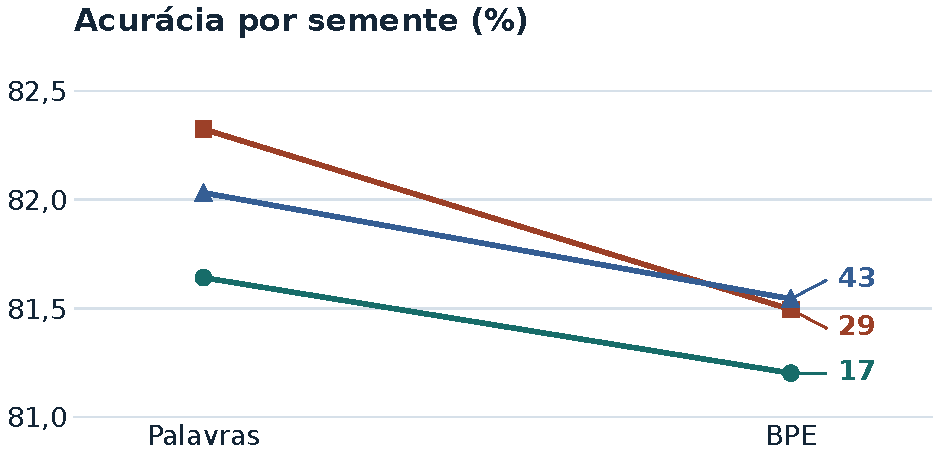
\includegraphics[width=\linewidth]{figuras/bpe_pareado.pdf}
\end{minipage}\hfill
\begin{minipage}[c]{.45\linewidth}
A diferença média é de \(-0,59\) ponto percentual para BPE. A cobertura
melhorou e a sequência ficou mais longa. Um filtro de cinco tokens pode
cobrir menos palavras, o que muda o contexto que ele observa. Esta
comparação estima o desempenho sob a taxa herdada e as larguras fixas.
\end{minipage}
\legendinha{Figura 3. Cada linha une a mesma semente sob as duas tokenizações.
Eixo vertical ampliado. \fonte{results/bpe/audit_metrics.json}{Métricas por execução}.}

\subsection{Pares sintéticos com a mesma contagem de palavras}
Escrevemos quatro pares antes da inferência e congelamos a lista em
\texttt{seminario/casos.json}. Verificamos a igualdade dos unigramas e
calculamos janelas de IDs de larguras 3, 4 e 5 com cada tokenizer.
Os seis checkpoints escolhidos no protocolo BPE foram executados em CPU.
Os números abaixo são médias de escores positivos antes de calibração.

\begin{tabularx}{\linewidth}{@{}Xrrrrl@{}}
\toprule
 & \multicolumn{2}{c}{\tabelahead{Palavras}} & \multicolumn{2}{c}{\tabelahead{BPE}} & \\
\cmidrule(lr){2-3}\cmidrule(lr){4-5}
\tabelahead{Par} & \tabelahead{A} & \tabelahead{B} & \tabelahead{A} & \tabelahead{B} &
\tabelahead{Trocas P/B}\\
\midrule
\LinhasPares
\bottomrule
\end{tabularx}
\legendinha{Tabela 8. Trocas de classe entre A e B em três sementes para palavras
e BPE. Aspectos e troca de blocos têm leitura mista. Os escores por semente,
IDs, janelas e hashes estão em \texttt{dados/pares\_resultados.json}.}

Em \textit{The movie is good, not bad}, a troca de \textit{good} e
\textit{bad} reduz o escore positivo médio nos dois tokenizadores.
Na semente 17, a própria frase A recebe \NegacaoPalavrasA{} com palavras
e \NegacaoBPEA{} com BPE. O limiar 0,5 dá classes diferentes para o mesmo
texto nas duas receitas treinadas.
No par da Seção~\ref{sec:ordem}, a troca muda a classe em todas as sementes
e inverte a leitura esperada. A Seção~\ref{sec:falhas} explica como o
controle com janelas iguais separa a reação local de um limite estrutural.

\newpage
\section{Confiança, comprimento e custo}
\label{sec:diagnosticos}
\subsection{O escore muda. A classe fica.}
Ajustamos uma temperatura \(\tau>0\) na amostra de calibração, minimizando
a CE. Com margem \(\Delta=z_+-z_-\), o escore passa de
\(\sigma(\Delta)\) a \(\sigma(\Delta/\tau)\). A transformação mantém o
sinal de \(\Delta\), de modo que a classe e as métricas de classificação
permanecem iguais no limiar de 50\%.

\begin{tabularx}{\linewidth}{@{}Xrrr@{}}
\toprule
\tabelahead{Modelo} & \tabelahead{Acurácia} & \tabelahead{F1 macro} &
\tabelahead{CE calibrada}\\
\midrule
\LinhasTeste
\bottomrule
\end{tabularx}
\legendinha{Tabela 6. Teste oficial, \(n=25.000\), com temperatura escolhida em
2.478 resenhas reservadas. A CE bruta está na Tabela 5.}

\medskip
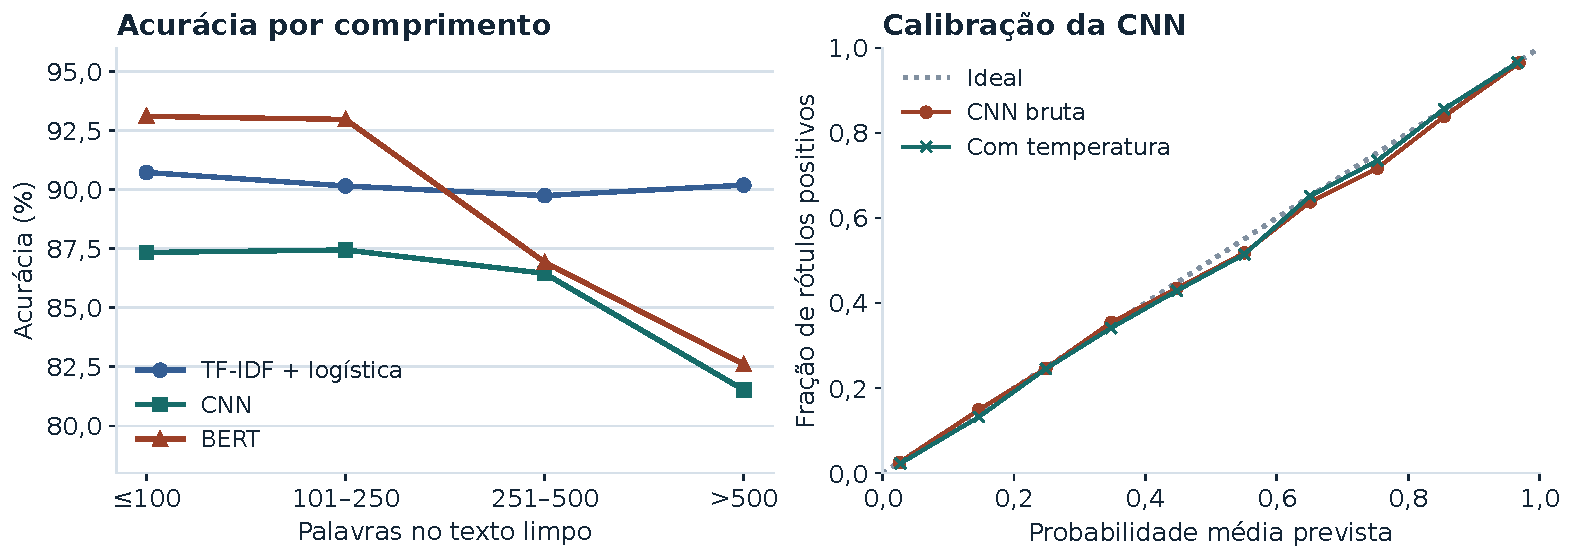
\includegraphics[width=\linewidth]{figuras/diagnostico_oficial.pdf}
\legendinha{Figura 3. À esquerda, as faixas de comprimento têm 3.246,
14.624, 5.285 e 1.845 resenhas. À direita, o eixo horizontal mostra a
probabilidade média prevista e o vertical mostra a fração de positivos
observada entre resenhas na mesma faixa de probabilidade. A diagonal
indica coincidência entre as duas medidas.}

A temperatura mudou pouco a CE da CNN, de 0,3040 para 0,3037. A acurácia
da CNN cai de 87,34\% nas resenhas de até cem palavras a 81,52\% acima
de 500. BERT também cai na faixa longa. O TF-IDF recebe o texto
completo e varia menos. Comprimento, conteúdo e recorte variam juntos.
\fonte{results/analysis/subgroup_metrics.csv}{Métricas por faixa}.

\subsection{O custo das três receitas originais}
\begin{tabularx}{\linewidth}{@{}Xlrr@{}}
\toprule
\tabelahead{Modelo} & \tabelahead{Dispositivo} & \tabelahead{Ajuste (s)} &
\tabelahead{Inferência (s)}\\
\midrule
\LinhasCusto
\bottomrule
\end{tabularx}
\legendinha{Tabela 7. A inferência soma as quatro divisões. O ajuste
do baseline inclui TF-IDF e seleção da regularização. Cada tempo vale para
o dispositivo e o orçamento da receita medida.}

\subsection{Ensaios complementares}
Em 64 enredos, o Qwen3-8B recebeu uma intervenção no bloco 28, após o
marcador de opinião. O próprio modelo reconheceu os dois tons-alvo em
55 enredos. Os resumos factuais coincidiram, mas uma opinião acrescentou
um cenário ausente da fonte \cite{qwen}.
\fonte{QWEN_EXPERIMENTO.md}{Protocolo de geração}.
O suplemento reúne 51 treinos de MLP e 880 condições sintéticas para
estudar \textit{double descent}.
\fonte{docs/CONEXOES_DISCIPLINA.md}{Guia dos mecanismos}.

\newpage
\section{Quando o modelo de aprendizagem profunda falha?}
\label{sec:falhas}
\subsection{A CNN reage à troca e inverte o sentido do contraste}
A termina em \textit{wonderful} (positiva) e B em \textit{terrible} (negativa).
Com três sementes por tokenizador, os seis treinos previram negativa em A e
positiva em B. O escore positivo foi de \PalavrasA{} a \PalavrasB{} com palavras
e de \BPEA{} a \BPEB{} com BPE, na média.
\href{https://costaleirbag.github.io/projeto-mae5920/\#slide-9}{Troca interativa A/B}.

\subsection{O máximo global apaga a posição entre janelas}
Uma frase repetida separa \textit{I loved the acting} de \textit{I hated the ending}.
Trocamos os dois blocos e verificamos que as janelas de 3, 4 e 5 IDs formam
os mesmos multiconjuntos nos dois tokenizadores. Cada filtro recebe as mesmas
janelas e conserva o mesmo máximo. Os logits coincidiram nos seis treinos.

Com os filtros congelados, guardamos dois picos por filtro. Uma cabeça linear
recebe menor e maior pico. A outra recebe os picos na ordem do texto. Guardar
a posição fez os escores de A e B diferirem. Em \NParesHumanos{} pares de
resenhas editadas, o acerto nas duas versões foi de \SemPosHumanos{} sem
posição e \ComPosHumanos{} com posição. \fonteatual{seminario/diagnosticos.md}{Método e três sementes}.

\subsection{O sentimento fora do IMDb}
Avaliamos os mesmos pesos em 1.000 frases de Amazon e 1.000 de Yelp, com
500 exemplos por classe em cada fonte \cite{kotzias}. Gênero e comprimento
mudam juntos em relação ao IMDb.

\begin{tabularx}{\linewidth}{@{}Xrrrrrr@{}}
\toprule
 & \multicolumn{3}{c}{\tabelahead{Palavras}} & \multicolumn{3}{c}{\tabelahead{BPE}}\\
\cmidrule(lr){2-4}\cmidrule(lr){5-7}
\tabelahead{Fonte} & \tabelahead{Acurácia} & \tabelahead{F1 macro} & \tabelahead{CE} &
\tabelahead{Acurácia} & \tabelahead{F1 macro} & \tabelahead{CE}\\
\midrule
\LinhasForaDominio
\bottomrule
\end{tabularx}
\legendinha{Tabela 11. Médias de três sementes em frases selecionadas por
polaridade clara. \fonteatual{seminario/dados/fora_dominio_resultados.json}{Resultados por semente}.}

Em \textit{The Room}, todos os treinos leram o elogio seguido de “No one”
como positivo. Os comentários de \textit{Baby} deram positivo. O de
\textit{Friday} deu negativo. \fonteatual{seminario/dados/fora_dominio_resultados.json}{Cinco casos sem rótulo}.

\subsection{Tom e fatos na geração do Qwen}
No bloco 28, somamos \(\alpha s v\) após \texttt{REVIEW}, com \(\alpha=-2,0,+2\).
A direção \(v\) compara as ativações médias para dois tons em 128 enredos.
O Qwen, como juiz automático, reconheceu os dois tons-alvo em 55 de 64 fontes.
\texttt{FACT} ficou igual. Em um caso, \texttt{REVIEW} inventou um cenário de
cidade pequena. \fonte{results/qwen_improved/fact_flag_reading.json}{Alertas factuais}.

\begin{thebibliography}{9}
\small
\setlength{\itemsep}{0pt}
\setlength{\parskip}{0pt}
\bibitem{maas} Maas, A. L. et al. \textit{Learning Word Vectors for Sentiment Analysis}.
ACL, 2011. \href{https://aclanthology.org/P11-1015/}{ACL Anthology}.
\bibitem{kim} Kim, Y. \textit{Convolutional Neural Networks for Sentence Classification}.
EMNLP, 2014. \href{https://aclanthology.org/D14-1181/}{ACL Anthology}.
\bibitem{sennrich} Sennrich, R., Haddow, B. e Birch, A.
\textit{Neural Machine Translation of Rare Words with Subword Units}. ACL, 2016.
\href{https://aclanthology.org/P16-1162/}{ACL Anthology}.
\bibitem{prince} Prince, S. J. D. \textit{Understanding Deep Learning}.
MIT Press, 2023. Caps. 6, 8, 9 e 10. \href{https://udlbook.github.io/udlbook/}{Livro e materiais}.
\bibitem{devlin} Devlin, J. et al. \textit{BERT: Pre-training of Deep Bidirectional
Transformers for Language Understanding}. NAACL, 2019.
\href{https://aclanthology.org/N19-1423/}{ACL Anthology}.
\bibitem{qwen} Yang, A. et al. \textit{Qwen3 Technical Report}, 2025.
\href{https://arxiv.org/abs/2505.09388}{arXiv:2505.09388}.
\bibitem{kotzias} Kotzias, D. et al. \textit{From Group to Individual Labels Using Deep Features}.
KDD, 2015. \href{https://doi.org/10.1145/2783258.2783380}{Artigo}.
\href{https://doi.org/10.24432/C57604}{Coleção UCI}.
\end{thebibliography}

\end{document}
